\documentclass[hyperref,]{ctexart}
\usepackage{lmodern}
\usepackage{amssymb,amsmath}
\usepackage{ifxetex,ifluatex}
\usepackage{fixltx2e} % provides \textsubscript
\ifnum 0\ifxetex 1\fi\ifluatex 1\fi=0 % if pdftex
  \usepackage[T1]{fontenc}
  \usepackage[utf8]{inputenc}
\else % if luatex or xelatex
  \ifxetex
    \usepackage{xltxtra,xunicode}
  \else
    \usepackage{fontspec}
  \fi
  \defaultfontfeatures{Mapping=tex-text,Scale=MatchLowercase}
  \newcommand{\euro}{€}
\fi
% use upquote if available, for straight quotes in verbatim environments
\IfFileExists{upquote.sty}{\usepackage{upquote}}{}
% use microtype if available
\IfFileExists{microtype.sty}{%
\usepackage{microtype}
\UseMicrotypeSet[protrusion]{basicmath} % disable protrusion for tt fonts
}{}
\ifxetex
  \usepackage[setpagesize=false, % page size defined by xetex
              unicode=false, % unicode breaks when used with xetex
              xetex]{hyperref}
\else
  \usepackage[unicode=true]{hyperref}
\fi
\usepackage[usenames,dvipsnames]{color}
\hypersetup{breaklinks=true,
            bookmarks=true,
            pdfauthor={谢益辉; 邱怡轩; 于淼},
            pdftitle={在R Markdown文档中使用中文},
            colorlinks=true,
            citecolor=blue,
            urlcolor=blue,
            linkcolor=magenta,
            pdfborder={0 0 0}}
\urlstyle{same}  % don't use monospace font for urls
\usepackage{color}
\usepackage{fancyvrb}
\newcommand{\VerbBar}{|}
\newcommand{\VERB}{\Verb[commandchars=\\\{\}]}
\DefineVerbatimEnvironment{Highlighting}{Verbatim}{commandchars=\\\{\}}
% Add ',fontsize=\small' for more characters per line
\usepackage{framed}
\definecolor{shadecolor}{RGB}{248,248,248}
\newenvironment{Shaded}{\begin{snugshade}}{\end{snugshade}}
\newcommand{\AlertTok}[1]{\textcolor[rgb]{0.94,0.16,0.16}{#1}}
\newcommand{\AnnotationTok}[1]{\textcolor[rgb]{0.56,0.35,0.01}{\textbf{\textit{#1}}}}
\newcommand{\AttributeTok}[1]{\textcolor[rgb]{0.77,0.63,0.00}{#1}}
\newcommand{\BaseNTok}[1]{\textcolor[rgb]{0.00,0.00,0.81}{#1}}
\newcommand{\BuiltInTok}[1]{#1}
\newcommand{\CharTok}[1]{\textcolor[rgb]{0.31,0.60,0.02}{#1}}
\newcommand{\CommentTok}[1]{\textcolor[rgb]{0.56,0.35,0.01}{\textit{#1}}}
\newcommand{\CommentVarTok}[1]{\textcolor[rgb]{0.56,0.35,0.01}{\textbf{\textit{#1}}}}
\newcommand{\ConstantTok}[1]{\textcolor[rgb]{0.00,0.00,0.00}{#1}}
\newcommand{\ControlFlowTok}[1]{\textcolor[rgb]{0.13,0.29,0.53}{\textbf{#1}}}
\newcommand{\DataTypeTok}[1]{\textcolor[rgb]{0.13,0.29,0.53}{#1}}
\newcommand{\DecValTok}[1]{\textcolor[rgb]{0.00,0.00,0.81}{#1}}
\newcommand{\DocumentationTok}[1]{\textcolor[rgb]{0.56,0.35,0.01}{\textbf{\textit{#1}}}}
\newcommand{\ErrorTok}[1]{\textcolor[rgb]{0.64,0.00,0.00}{\textbf{#1}}}
\newcommand{\ExtensionTok}[1]{#1}
\newcommand{\FloatTok}[1]{\textcolor[rgb]{0.00,0.00,0.81}{#1}}
\newcommand{\FunctionTok}[1]{\textcolor[rgb]{0.00,0.00,0.00}{#1}}
\newcommand{\ImportTok}[1]{#1}
\newcommand{\InformationTok}[1]{\textcolor[rgb]{0.56,0.35,0.01}{\textbf{\textit{#1}}}}
\newcommand{\KeywordTok}[1]{\textcolor[rgb]{0.13,0.29,0.53}{\textbf{#1}}}
\newcommand{\NormalTok}[1]{#1}
\newcommand{\OperatorTok}[1]{\textcolor[rgb]{0.81,0.36,0.00}{\textbf{#1}}}
\newcommand{\OtherTok}[1]{\textcolor[rgb]{0.56,0.35,0.01}{#1}}
\newcommand{\PreprocessorTok}[1]{\textcolor[rgb]{0.56,0.35,0.01}{\textit{#1}}}
\newcommand{\RegionMarkerTok}[1]{#1}
\newcommand{\SpecialCharTok}[1]{\textcolor[rgb]{0.00,0.00,0.00}{#1}}
\newcommand{\SpecialStringTok}[1]{\textcolor[rgb]{0.31,0.60,0.02}{#1}}
\newcommand{\StringTok}[1]{\textcolor[rgb]{0.31,0.60,0.02}{#1}}
\newcommand{\VariableTok}[1]{\textcolor[rgb]{0.00,0.00,0.00}{#1}}
\newcommand{\VerbatimStringTok}[1]{\textcolor[rgb]{0.31,0.60,0.02}{#1}}
\newcommand{\WarningTok}[1]{\textcolor[rgb]{0.56,0.35,0.01}{\textbf{\textit{#1}}}}
\RecustomVerbatimEnvironment{Highlighting}{Verbatim}{commandchars=\\\{\},formatcom=\xeCJKVerbAddon}
\usepackage{graphicx,grffile}
\makeatletter
\def\maxwidth{\ifdim\Gin@nat@width>\linewidth\linewidth\else\Gin@nat@width\fi}
\def\maxheight{\ifdim\Gin@nat@height>\textheight\textheight\else\Gin@nat@height\fi}
\makeatother
% Scale images if necessary, so that they will not overflow the page
% margins by default, and it is still possible to overwrite the defaults
% using explicit options in \includegraphics[width, height, ...]{}
\setkeys{Gin}{width=\maxwidth,height=\maxheight,keepaspectratio}
\setlength{\emergencystretch}{3em}  % prevent overfull lines
\providecommand{\tightlist}{%
  \setlength{\itemsep}{0pt}\setlength{\parskip}{0pt}}
\setcounter{secnumdepth}{5}

\title{在R Markdown文档中使用中文}
\author{谢益辉 \and 邱怡轩 \and 于淼}
\date{}



% Redefines (sub)paragraphs to behave more like sections
\ifx\paragraph\undefined\else
\let\oldparagraph\paragraph
\renewcommand{\paragraph}[1]{\oldparagraph{#1}\mbox{}}
\fi
\ifx\subparagraph\undefined\else
\let\oldsubparagraph\subparagraph
\renewcommand{\subparagraph}[1]{\oldsubparagraph{#1}\mbox{}}
\fi

\begin{document}
\maketitle

{
\setcounter{tocdepth}{2}
\tableofcontents
}
\hypertarget{ux5f15ux8a00}{%
\section{引言}\label{ux5f15ux8a00}}

中文LaTeX文档并非难题。当然这句话得站在巨人 \href{http://ctex.org}{CTeX}
的肩膀上才能说,它让我们只需要一句

\begin{Shaded}
\begin{Highlighting}[]
\BuiltInTok{\textbackslash{}documentclass}\NormalTok{\{}\ExtensionTok{ctexart}\NormalTok{\} }\CommentTok{% 或者ctexrep/ctexbook}
\end{Highlighting}
\end{Shaded}

或者

\begin{Shaded}
\begin{Highlighting}[]
\BuiltInTok{\textbackslash{}usepackage}\NormalTok{\{}\ExtensionTok{ctex}\NormalTok{\}}
\end{Highlighting}
\end{Shaded}

就轻松搞定中文LaTeX排版问题。

\hypertarget{ux5b57ux4f53ux548cux9009ux9879}{%
\section{字体和选项}\label{ux5b57ux4f53ux548cux9009ux9879}}

LaTeX包\href{http://ctan.org/pkg/ctex}{\textbf{ctex}}支持若干种字体选项,如果你是\textbf{ctex}老用户,请注意这里我们要求的最低版本是2.2,你可能需要升级你的LaTeX包。从版本2.0开始,\textbf{ctex}支持根据不同操作系统自动选择中文字体,简直是为人类进步作出了巨大贡献,我们再也不必费尽口舌向用户解释``啊,你用Windows啊,那么你该使用什么字体;啊,你用Mac啊,又该如何如何''。

下面的YAML元数据应该能满足多数用户的需求,主要设置两项参数:文档类为\texttt{ctexart}(当然也可以是别的类),输出格式为\texttt{rticles::ctex},其默认LaTeX引擎为XeLaTeX(真的,别纠结你的旧爱PDFLaTeX了)。

\begin{Shaded}
\begin{Highlighting}[]
\OtherTok{---}
\FunctionTok{documentclass:}\AttributeTok{ ctexart}
\FunctionTok{output:}\AttributeTok{ rticles::ctex}
\OtherTok{---}
\end{Highlighting}
\end{Shaded}

\texttt{rticles::ctex}的参数都是普通的\texttt{pdf\_document}参数,参见文档\textbf{rmarkdown}包的文档,这里就不赘述了。

Windows和Mac用户应该都已经有自带的中文字体了。Linux用户可以考虑
\href{http://ctan.org/pkg/fandol}{Fandol字体},它号称是免费的,不过我们也没太搞清楚它的来头。如果你不想操心这些问题,我们强烈建议你卸载你当前的
LaTeX 套装(TeX Live 或 MiKTeX 或 MacTeX),换上
TinyTeX,一切将会自动化搞定。

\begin{Shaded}
\begin{Highlighting}[]
\NormalTok{devtools}\OperatorTok{::}\KeywordTok{install_github}\NormalTok{(}\KeywordTok{c}\NormalTok{(}\StringTok{'rstudio/rmarkdown'}\NormalTok{, }\StringTok{'yihui/tinytex'}\NormalTok{))}
\NormalTok{tinytex}\OperatorTok{::}\KeywordTok{install_tinytex}\NormalTok{()}
\end{Highlighting}
\end{Shaded}

\hypertarget{rux4ee3ux7801ux6bb5}{%
\section{R代码段}\label{rux4ee3ux7801ux6bb5}}

R代码用R
Markdown的语法嵌入,即三个反引号开始一段代码\texttt{\textasciigrave{}\textasciigrave{}\textasciigrave{}\{r\}}和三个反引号\texttt{\textasciigrave{}\textasciigrave{}\textasciigrave{}}
结束一段代码:

\begin{Shaded}
\begin{Highlighting}[]
\KeywordTok{options}\NormalTok{(}\DataTypeTok{digits =} \DecValTok{4}\NormalTok{)}
\NormalTok{fit =}\StringTok{ }\KeywordTok{lm}\NormalTok{(dist }\OperatorTok{~}\StringTok{ }\NormalTok{speed, }\DataTypeTok{data =}\NormalTok{ cars)}
\KeywordTok{coef}\NormalTok{(}\KeywordTok{summary}\NormalTok{(fit))}
\end{Highlighting}
\end{Shaded}

\begin{verbatim}
##             Estimate Std. Error t value  Pr(>|t|)
## (Intercept)  -17.579     6.7584  -2.601 1.232e-02
## speed          3.932     0.4155   9.464 1.490e-12
\end{verbatim}

\begin{Shaded}
\begin{Highlighting}[]
\NormalTok{b =}\StringTok{ }\KeywordTok{coef}\NormalTok{(fit)}
\end{Highlighting}
\end{Shaded}

上面回归方程中的斜率是3.9324,完整的回归方程为:\[ Y = -17.5791 + 3.9324x\]

画图当然也是木有问题的啦,想画就说嘛,不说我怎么知道你想画呢?

\begin{Shaded}
\begin{Highlighting}[]
\KeywordTok{par}\NormalTok{(}\DataTypeTok{mar =} \KeywordTok{c}\NormalTok{(}\DecValTok{4}\NormalTok{, }\DecValTok{4}\NormalTok{, }\FloatTok{.1}\NormalTok{, }\FloatTok{.1}\NormalTok{), }\DataTypeTok{las =} \DecValTok{1}\NormalTok{)}
\KeywordTok{plot}\NormalTok{(cars, }\DataTypeTok{pch =} \DecValTok{19}\NormalTok{)}
\KeywordTok{abline}\NormalTok{(fit, }\DataTypeTok{col =} \StringTok{'red'}\NormalTok{)}
\end{Highlighting}
\end{Shaded}

\begin{figure}
\centering
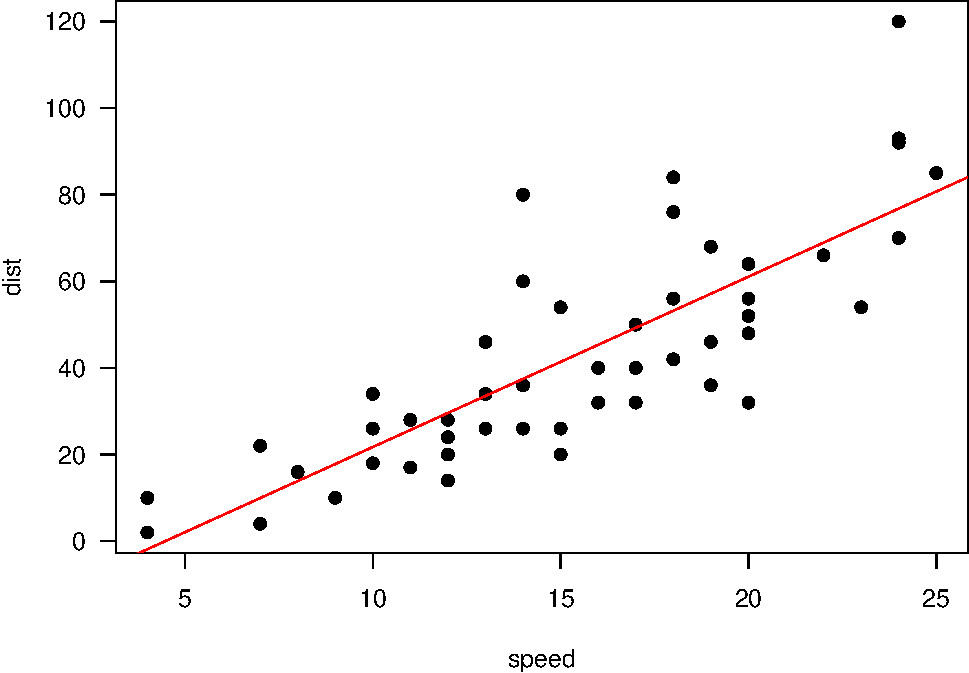
\includegraphics{在R-Markdown文档中使用中文_files/figure-latex/scatter-1.pdf}
\caption{cars数据散点图以及回归直线。}
\end{figure}

请不要问我为什么图浮动到下一页去了,这么初级的LaTeX问题问出来信不信我扁你。

\hypertarget{ux6e90ux4ee3ux7801ux63a7}{%
\section{源代码控}\label{ux6e90ux4ee3ux7801ux63a7}}

这里提供的rticles模板可能由于种种原因不能满足客官的要求,LaTeX用户就是这样永无止境地调格式(唉,跟Word用户到底有啥区别呢)。若真是需要调整,你可以复制一份默认模板去改,如前面所说,本文档的模板是\texttt{rticles::ctex\_template()},它是一个文本文件。若熟悉LaTeX的话一看就明白,只不过里面有些Pandoc变量而已;若不熟悉LaTeX我们在这里说了也白说,花几天时间好好啃一啃LaTeX入门手册吧。

本文档所用的模板是从Pandoc默认LaTeX模板基础上做了少许改动而来的:\url{https://github.com/yihui/pandoc-templates/blob/ctex/default.latex}
具体改动从GIT提交消息日志中可以看到,主要就是去掉了mathspec包和hyperref包。

\hypertarget{ux5c0fux7ed3}{%
\section{小结}\label{ux5c0fux7ed3}}

事实证明我们可以理直气壮地通过XeLaTeX将中文R
Markdown转化为PDF文档,麻麻再也不用担心我的论文满屏幕都是反斜杠,朕养完小白鼠之后终于不必先折腾三个小时LaTeX再开始写实验报告了:打开RStudio,菜单File
\textgreater{} New File \textgreater{} R Markdown,然后从模板中选择CTeX
Documents,搞定。

\end{document}
